% +--------------------------------------------------------------------+
% | Sample Chapter 2
% +--------------------------------------------------------------------+

\cleardoublepage

% +--------------------------------------------------------------------+
% | Replace "This is Chapter 2" below with the title of your chapter.
% | LaTeX will automatically number the chapters.
% +--------------------------------------------------------------------+

\chapter{Estado del arte}
\label{makereference2}
Para que esta aplicación sea usable e interactiva, en esta sección de la memoria procederemos a 
realizar un estudio de las posibles tecnologías que nos permitan llevar a cabo nuestros objetivos, 
tales como la realidad aumentada, las distintas fuentes de información y algunas
técnicas de recomendación. 
\section{Realidad Aumentada}
\label{makereference2.1}

\begin{quote}
``
La realidad aumentada nos permite añadir capas de información visual sobre el 
mundo real que nos rodea, utilizando la tecnología, dispositivos como pueden ser 
nuestros propios teléfonos móviles. Esto nos ayuda a generar experiencias que aportan
un conocimiento relevante sobre nuestro entorno, y además recibimos esa información en 
tiempo real. Mediante la realidad aumentada el mundo virtual se entremezcla con el mundo 
real, de manera contextualizada, y siempre con el objetivo de comprender mejor todo lo que 
nos rodea.
''
\end{quote}


\begin{figure}[htb]
    \centering
    \makebox[0pt][c]{%
    \begin{minipage}[b]{0.5\linewidth}
    \centering
      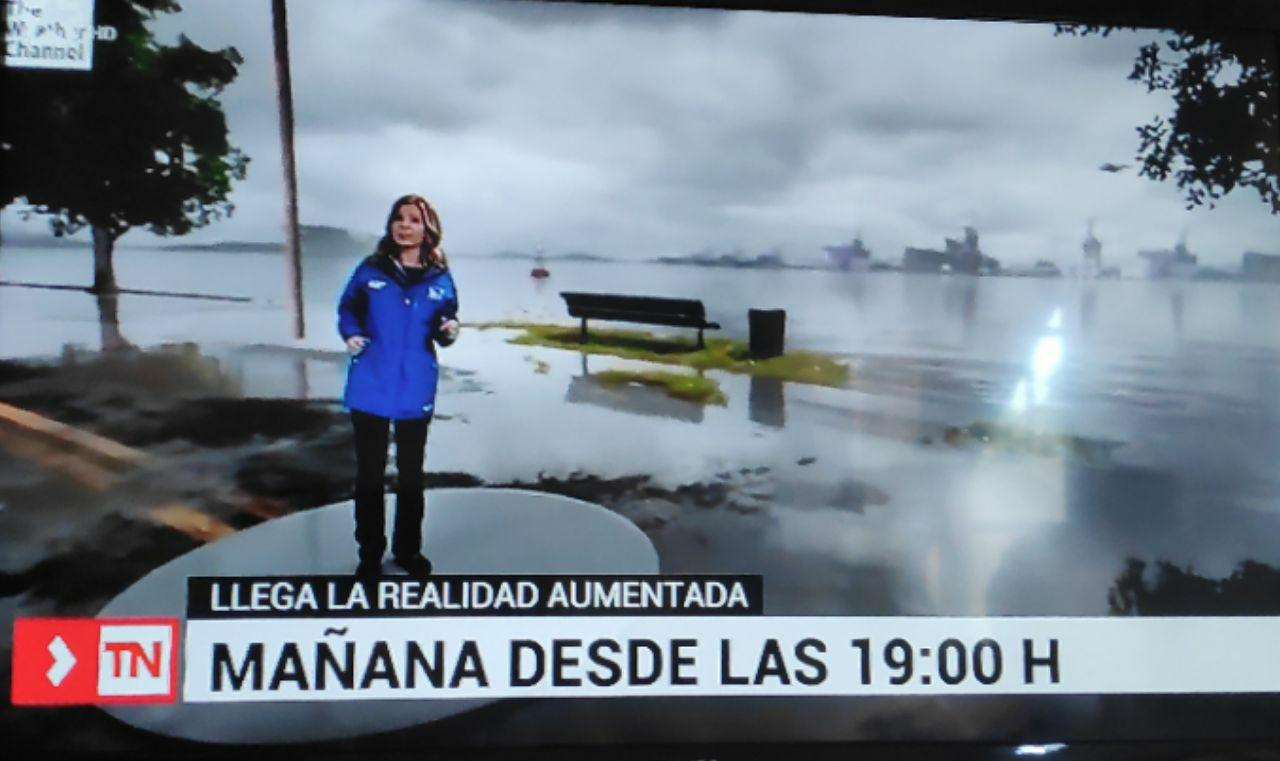
\includegraphics[scale=0.2]{figures/chapter-2/televisionAR-1.jpg}
      \caption{Telemadrid anuncia el uso de RA en las elecciones de 2019}
      \label{fig:sva}
    \end{minipage}%
    \hspace{0.3cm}
    \begin{minipage}[b]{0.5\linewidth}
    \centering
     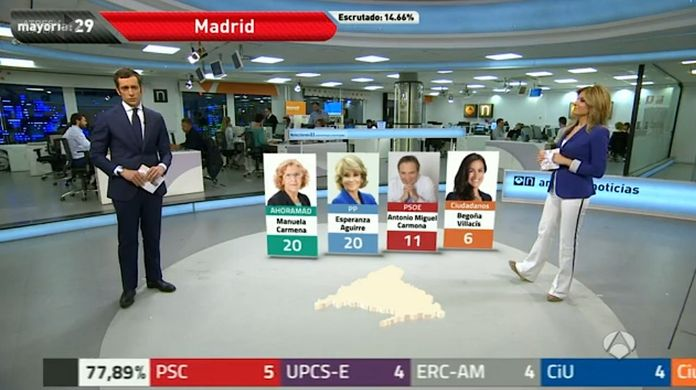
\includegraphics[scale=0.3]{figures/chapter-2/televisionAR-3.jpg}
      \caption{Antena 3 usa RA para las elecciones del ayuntamiento de Madrid}
    \label{fig:svb}
    \end{minipage}%
    }%
\end{figure}


La realidad aumentada se aplica a diversas áreas como seguridad, logística, sanidad, ocio, etc...
 Se puede aplicar a tantas disciplinas como podamos imaginar y no sólo se ha convertido en una herramienta útil, sino que es una tecnología atractiva
 y además signo de modernidad. Por estas razones actualmente vemos ejemplos como el de las televisiones, que compiten por aplicarla a sus programas
 y presumir de dar el mejor servicio a sus espectadores como vemos en las Figuras~\ref{fig:sva} y \ref{fig:svb}. Con esta situación podemos por tanto estar de acuerdo
 en que es una tecnología en auge actualmente. 


Los smartphones son los dispositivos que más interaccionan con esta tecnología, ya que prácticamente todas las personas poseen uno
 y están dotados de un amplio abanico de sensores necesarios para su correcto funcionamiento. Por esto elegimos este tipo de dispositivos para nuestro
 proyecto ya que, esta tecnología, aporta un gran valor añadido a nuestra aplicación, incluso siendo el grueso de la misma. 

 La realidad aumentada en cualquier dispositivo se basa en dónde nos encontramos y hacia donde estamos mirando, es decir, si usamos la cámara del teléfono,
 según a donde estemos mirando a través de ésta, la realidad aumentada superpondrá objetos virtuales o información a nuestra realidad, con un cierto tamaño y una cierta posición
 basándose en las medidas de lo que vemos a través de nuestra cámara. Por ejemplo, la famosa aplicación de Pokemon Go, que superpone la imagen de un pokemon a la realidad
 que vemos con la cámara para que podamos atraparlo, haciendo así que su uso sea más interactivo y visual para el usuario, como podemos observar en las Figuras \ref{fig:pokemon}, \ref{fig:libertystatue} y \ref{fig:measure}.

 \begin{figure}[H]
    \centering
    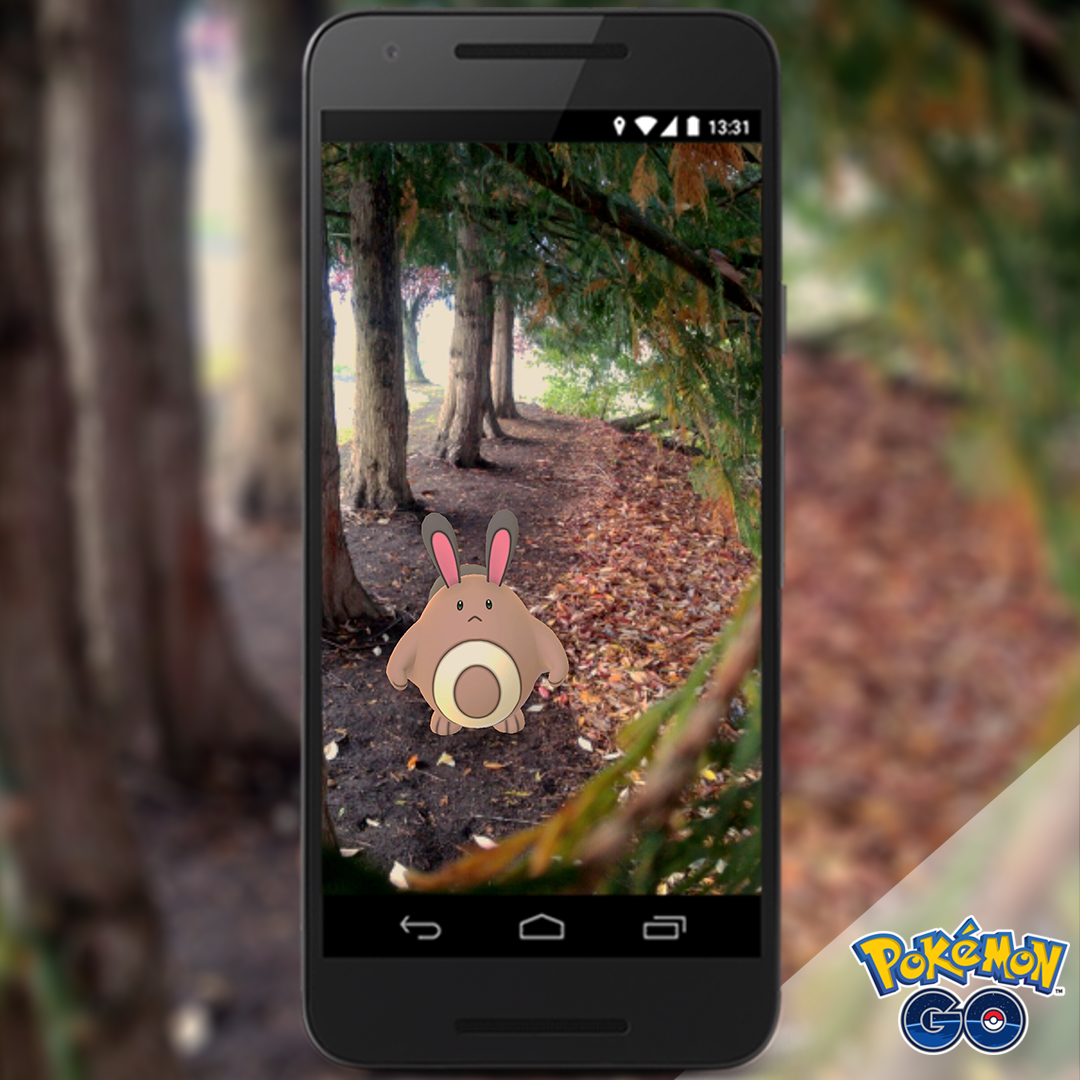
\includegraphics[width=4in]{figures/chapter-2/pokemongo.png}
    \caption{RA en Pokemon Go}
    \label{fig:pokemon}
\end{figure}

\begin{figure}[htb]
    \centering
    \makebox[0pt][c]{%
    \begin{minipage}[b]{0.5\linewidth}
    \centering
      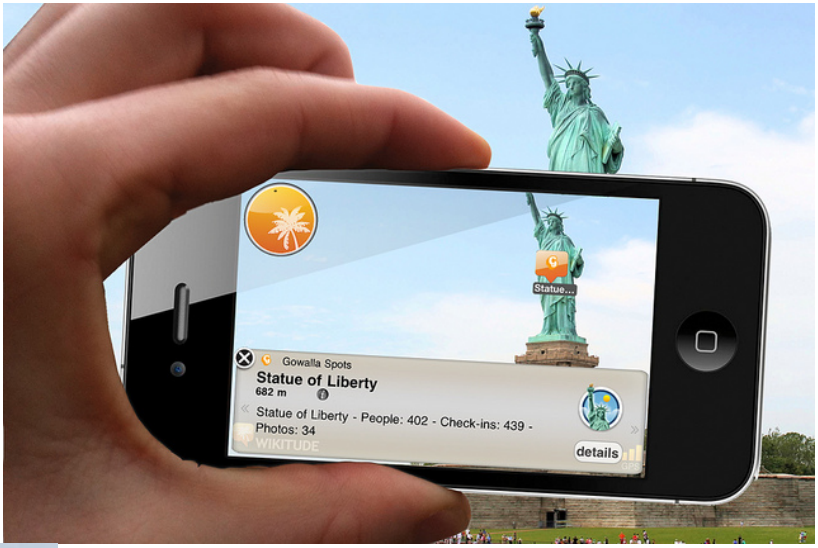
\includegraphics[scale=0.2]{figures/chapter-2/ralibertystatue.png}
      \caption{RA para zonas turísticas}
      \label{fig:libertystatue}
    \end{minipage}%
    \hspace{0.3cm}
    \begin{minipage}[b]{0.5\linewidth}
    \centering
     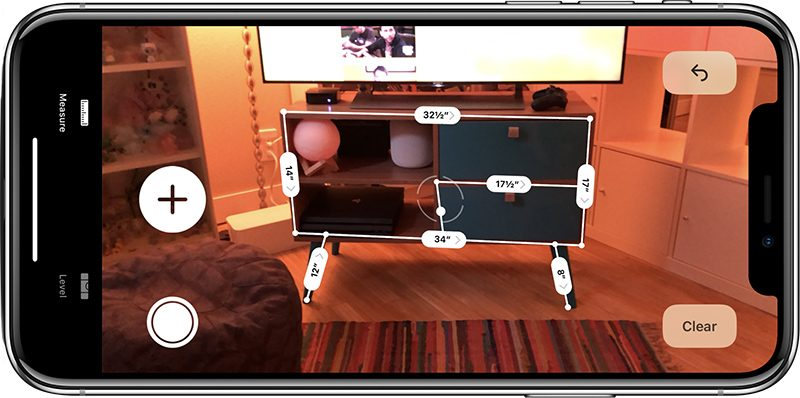
\includegraphics[scale=0.3]{figures/chapter-2/rameasure.jpg}
      \caption{RA para mediciones}
    \label{fig:measure}
    \end{minipage}%
    }%
\end{figure}

\subsection{Tecnologías actuales}
\label{makereference2.1.1}
A continuación, describiremos las distintas tecnologías que hemos investigado para la implementación de la Realidad Aumentada.
\begin{itemize}
    \item ARCore\cite{arcore}: esta plataforma creada por Google para desarrollar aplicaciones de
 realidad aumentada con soporte para Android, Android NDK, iOS,
 Unity y Unreal Engine, aunque las funcionalidades que se ofrecen
 para iOS y Unity for iOS se limitan a Cloud Anchors. Los anchors
 son herramientas que permiten que objetos virtuales aparezcan en un lugar
 captado por la cámara de nuestro dispositivo, estos son compartidos
 en la nube para que multitud de dispositivos disfruten de la misma
 experiencia, aquellos que posean iOS podrán usarlos utilizando ARKit.

Tiene una curva de aprendizaje media y con su versión 1.5 demuestra una
 estabilidad interesante respecto a su reciente creación. Cabe destacar
 que no todos los dispositivos son compatibles. Esto depende de que las
 empresas que desarrollan estos dispositivos cumplan unos requisitos
 para asegurar que la experiencia con ARCore es la adecuada y de la
 versión del sistema operativo.
ARCore usa tres características a través de la cámara del dispositivo:
 \begin{itemize}  
     \item Motion tracking: permite al dispositivo conocer la posición relativa del mundo.
     \item Environmental understanding: permite al dispositivo detectar el tamaño y localización de todos los tipos de superficies.
     \item Light estimation: permite al dispositivo estimar las condiciones de luz del entorno actual.
 \end{itemize}

\item ARKit\cite{arkit}: es una librería desarrollada por Apple que podemos utilizar para crear 
experiencias de realidad aumentada persistente y compartirlas entre distintos dispositivos iOS. 
Detecta imágenes 2D incluso en movimiento y objetos 3D. Esta tecnología se basa en la odometría visual inercial, esta es capaz 
de reconocer las imágenes que capta la cámara y la forma en la que la luz se refleja 
en los diferentes elementos que aparecen para obtener un mapa 3D del entorno y, calcular las distancias que hay entre los diferentes objetos 
desde la posición del dispositivo. Tras iniciar la realidad aumentada con ARKit, nuestro dispositivo crea un entorno virtual donde nuestro
dispositivo representa la coordenada (0,0,0), con los tres ejes, el horizontal, vertical y el de profundidad, pero también es necesario otro eje,
el eje W que representa la rotación del dispositivo. En la Figura \ref{fig:arkit} se puede observar cómo cambia el elemento virtual según como situemos nuestro
smartphone.

\begin{figure}[H]
    \centering
    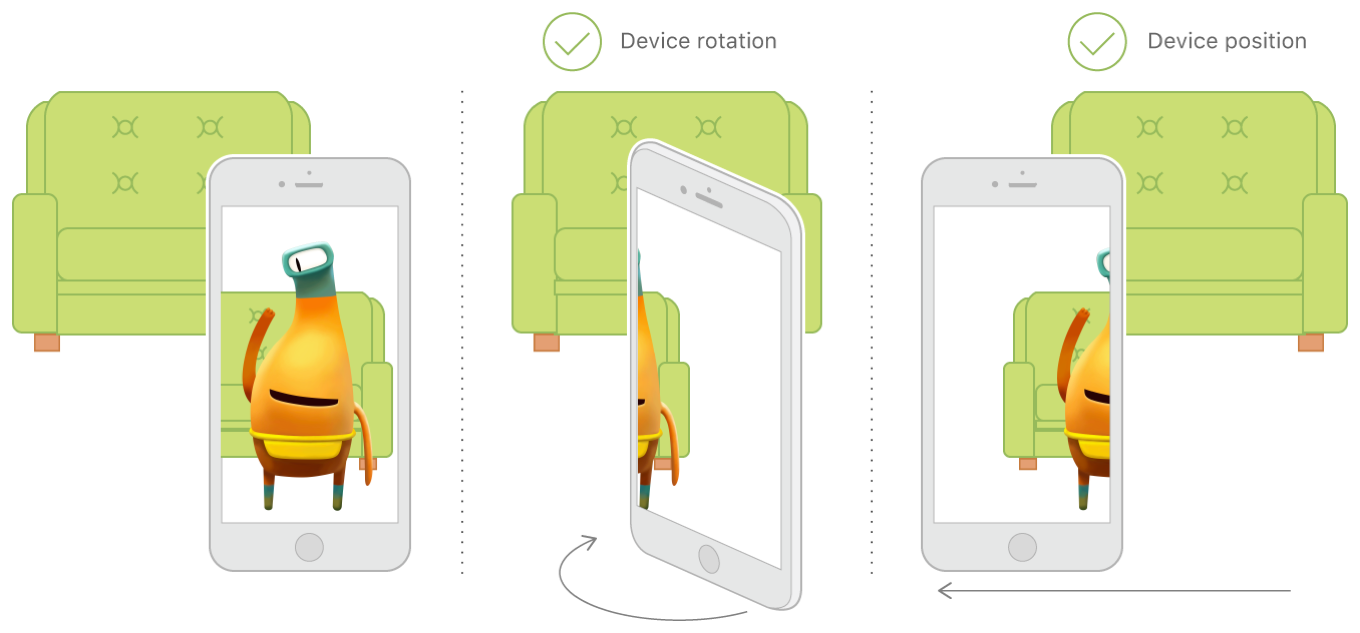
\includegraphics[width=4in]{figures/arkit.png}
    \caption{RA en ARKit}
    \label{fig:arkit}
\end{figure}



\item Wikitude\cite{wikitude}:
es un kit de desarrollo para realidad aumentada con soporte para Android, iOS, Unity, Cordova, Xamarin, Titanium y React Native.
Su licencia es de pago, aunque hay versiones limitadas gratuitas.
Utiliza ARCore o ARKit cuando los dispositivos lo soportan y en caso contrario utiliza tecnología de Wikitude
 para que el número de dispositivos compatibles sea mayor. Algunas de las tecnologías que soporta Wikitude son la geolocalización, el reconocimiento 
 de imágenes y el reconocimiento en la nube. Para entender cómo funciona este SDK tenemos que describir tres términos básicos fundamentales:
\begin{itemize}
    \item Target: conjunto de datos extraídos de una imagen, empleados por un rastreador al reconocerla para realizar alguna acción.
    \item Target Collection: es un conjunto de targets empleado por el rastreador para reconocer imágenes en el mundo real.
    \item Client Tracker: rastreador que usa la cámara para analizar objetos 2D, analiza el Target Collection y busca similitudes con la imagen reconocida.
\end{itemize}

\item Vuforia\cite{vuforia}:
Kit de desarrollo para realidad aumentada con soporte para Android, iOS, UWP y Unity.
Su licencia es de pago, aunque puede usarse gratis para el desarrollar y probar. Su integración con Unity permite crear aplicaciones y juegos 
para que sean usados en Android y iOS simplemente arrastrando y soltando elementos. Usa un seguimiento basado en marcadores, los marcadores son las imágenes u objetos
reconocidos por la aplicación para desencadenar la visualización del contenido virtual
sobre su posición en la vista de la cámara.
Los Image Targets u objetivos de imagen, son un tipo específico de marcador, son imágenes que se registran manualmente en la aplicación y que pueden ser guardadas en un Cloud,
reduciendo así el peso de tener las imágenes a reconocer en el dispositivo.
También se puede realizar un seguimiento sin marcado, basado en el GPS o en un giroscopio para insertar modelos de objetos virtuales en la realidad que capta la cámara.

\item ViroReact\cite{viroreact}:
Plataforma para construir aplicaciones con realidad aumentada usando React Native.
 Utiliza ARKit y ARCore para dotar a las aplicaciones de una experiencia de Realidad Aumentada sin
 utilizar código distinto y con una curva de aprendizaje fácil. Al basarse en React
 Native que no tiene versión estable provoca problemas con las versiones de dependencias,
 configuraciones tediosas y largas compilaciones.
Es un software privativo gratuito.

\item Expo AR\cite{expoar}:
Es un conjunto de librerías escritas de forma nativa para cada plataforma, proporcionando acceso a la funcionalidad del sistema del
dispositivo (como pueden ser la cámara, notificaciones emergentes, contactos, almacenamiento local y otro tipo de hardware) desde JavaScript. Está 
desarrollado para suavizar las diferencias entre plataformas lo máximo posible, consiguiendo que los proyectos que se realicen sean muy portables ya que pueden
ejecutarse en cualquier entorno nativo que contengo el SDK de Expo.
También proporciona componentes de interfaz de usuario para manejar una variedad de casos de uso que casi todas las aplicaciones móviles tienen que cubrir pero no están
construidas en el núcleo de React Native, por ejemplo, iconos, vistas borrosas (aquellas que aparecen de fondo para que el usuario se centre más en los elementos que están superpuesto a la imagen), etc.
\end{itemize}


\section{Fuentes de información}
\label{makereference2.2}
Como nuestra aplicación muestra información sobre las películas que se recomiendan y que los usuarios han guardado, hemos
tenido que investigar de qué fuentes de información podríamos obtener estos datos tan relevantes. Con la finalidad de extraer
estos datos, guardarlos en contenedores de datos y por último, representarlos ante los usuarios.
\begin{itemize}
    \item FilmAffinity\cite{filmaffinity}: es una de las páginas webs más relevantes para obtener información sobre películas y series, además de críticas y valoraciones de profesionales y sugerencias personalizadas.
    Esta página fue creado al principio, con la única intención de ser un sistema recomendador, el cual es un factor que nos beneficia ya que podemos asegurarnos de que sus datos están preparados para la recomendación.
    Por otro lado, la página ofrece dos idiomas, español e inglés, otro factor a favor pues en nuestra aplicación se usa el inglés como idioma primario y el español es la que usamos para comunicarnos. Sin embargo, la página por 
    hacer críticas bastantes serias y profesionales, la tendencia de valoraciones suelen ser bajas.
    \item MovieLens\cite{movielens}: una fuente de información, quizás menos conocida que FilmAffinity y que IMDB pero que ofrece sugerencias personalizadas y posibilidad de valorar. Se trata de un sistema de recomendación basado en una técnica de recomendación 
    llamado filtrado colaborativo\cite{filtradocolaborativo}, que es una técnica candidata a usar en nuestra aplicación. Los datos que nos proporciona está en inglés.
    \item IMDB\cite{imdb}: se trata de una base de datos online donde se guardan la información relacionada con las películas y series. Es una de las páginas mundialmente más usadas en estos aspectos.
    Actualmente, le pertenece a una de las empresas que más nubes tienen en el mundo, Amazon, por lo que se puede asegurar su fiabilidad. Su idioma está en inglés.
    \item Rotten Tomatoes\cite{rottentomatoes}: es una web donde usuarios y
     críticos profesionales puntúan películas y espectáculos televisivos.
    La puntuación es representada con tomates frescos si el 60\% de las
     críticas son positivas y si es menor de ese porcentaje es representada con
     un tomate podrido explotando.
    Existen certificados de una distinción especial si además, cumplen más
     requisitos:
     \begin{itemize}
         \item Una puntuación constante en el Tomatómetro de 75\% o más.
         \item Al menos cinco reseñas de los mejores críticos.
         \item Las películas en ``wide release'' deben tener un mínimo de 80 revisiones.
         \item Las películas en ``limited release'' deben tener un mínimo de 40 revisiones.
         \item Solo las temporadas individuales de un programa de televisión son certificables, y cada uno ha de tener un mínimo de 20 revisiones.
     \end{itemize}
    Estos certificados además de que tienen que ser valorados por un grupo de jurados, pueden además ser retirados una vez que esta película o serie
    no sea capaz de mantener los requisitos.
\end{itemize}

\section{Técnicas de recomendación}
\label{makereference2.3}

\begin{quote}
``
Un sistema de recomendación es un sistema inteligente que proporciona a los usuarios una serie de 
sugerencias personalizadas (\textbf{recomendaciones}) sobre un determinado tipo de elementos (\textbf{items}). Los 
sistemas de recomendación estudian las características de cada usuario y mediante un procesamiento 
de los datos, encuentra un subconjunto de items que pueden resultar de interés para el usuario. 
''
\end{quote}

Entre los distintos tipos de técnicas de recomendación que hemos encontrado en Internet, vamos a destacar dos, pues son las que mejor se asemejan a nuestra situación.

\begin{itemize}
    \item Filtrado Colaborativo\cite{filtradocolaborativo}: esta técnica de recomendación se basa en buscar usuarios que tienen preferencias similares, es decir, se basa en las valoraciones que han dado otros usuarios a los elementos.
    \item Filtrado basado en el contenido\cite{filtradocontenido}: al usuario se le recomendará aquella información que le ha interesado en el pasado, es decir, se le mostrarán elementos similares, independientemente de lo que opinen otros usuarios. 
\end{itemize} 

\begin{figure}[H]
    \centering
    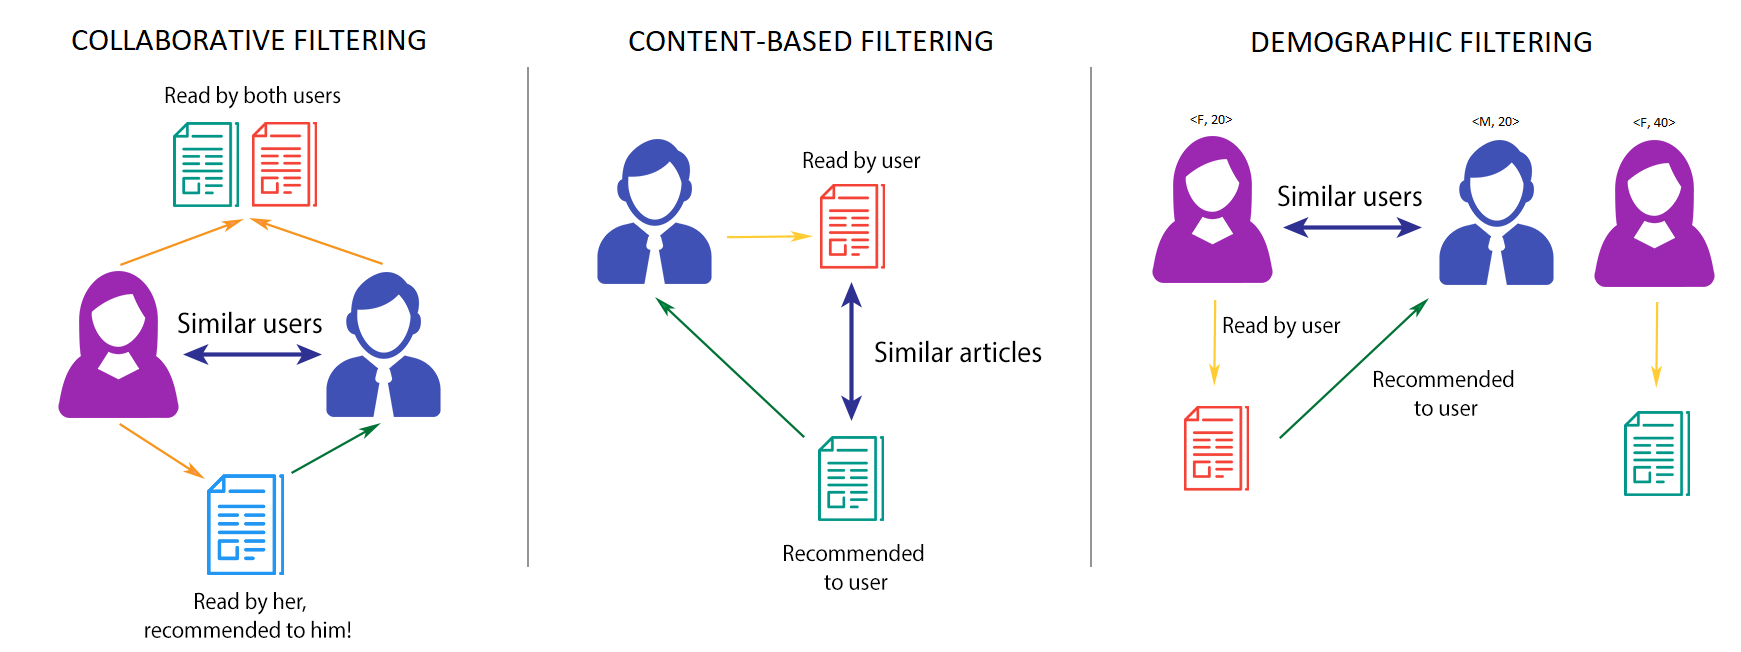
\includegraphics[width=3in, angle=0]{figures/chapter-2/recommendation_systems.png}
    \caption{Tipos de sistemas de recomendación \cite{imagefilters}}
\end{figure}


En este capítulo hemos podido conocer de primera mano la tecnología que representa el grueso de nuestra aplicación, la realidad aumentada. Se han descrito 
los distintos tipos de librerías que hemos investigado para su implementación. También las diferentes páginas web de las que podríamos obtener la información necesaria
para nutrir a nuestra aplicación y a nuestros usuarios. Finalmente hemos incluido un breve resumen de las técnicas de recomendación que más se ajustan a nuestra aplicación, en los próximos capítulos
se tratará más a fondo este tema, cuando se haya descrito con más detalle nuestra aplicación.

